\chapter{晶体I：理想晶体与金属}\label{ch:b1:crystals-metals}

铜丝可以拉得比头发还细而不断；
一块盐在锤下却会碎裂。铁匠把一根铁条加热至
发光，锤打后投入水中，
取出的铁条比入水前硬得多。这些性质的差异，
源于固体中原子的堆积方式。大多数固体是\omterm{def:b1:crystals-metals:crystal}{晶体}：
其原子位于一种不断重复的图案上，
在各个方向上完全相同地重复无数次。本章描述这类图案，
计算其中的原子数，测量它们堆积的紧密程度以及原子之间空隙的位置，
并利用所得结果来理解金属与合金。
下一章将同样的方法应用于
离子型、共价型和分子型固体。

\begin{recall}
金属很容易失去\omterm{def:b1:quantum-numbers:configuration}{价电子}：它们的电离能
和\omterm{def:b1:periodicity:electronegativity}{电负性}都较低（见\cref{ch:b1:periodicity}）。
原子半径已在\cref{def:b1:periodicity:radius}中定义。
密度是物理学中学过的性质，此处直接使用：$\rho = m/V$。
\end{recall}

\begin{omfigure}

\includegraphics[width=0.55\linewidth]{images/book2/ai/b1-05-blacksmith.jpg}

{\small 一位铁匠正在锻打钢材。加热后发橙光的铁
其\omterm{def:b1:crystals-metals:crystal}{晶体}结构与室温下的铁不同，
并且能溶解更多的碳（周末问题）。}
\end{omfigure}

\section{理想晶体模型}

\begin{definition}[晶体、非晶态固体、理想晶体]\label{def:b1:crystals-metals:crystal}
\emph{晶体}\index{晶体}是粒子（原子、离子或分子）按
在三维空间中\omterm{def:b1:periodicity:table}{周期}性重复的图案排列而成的固体。
不具有这种长程有序性的固体称为
\emph{非晶态固体}\index{非晶态固体}（如玻璃、大多数塑料）。
\emph{理想晶体模型}\index{理想晶体模型}把晶体看作
无限延伸、无缺陷的：没有缺失或多余的原子，
没有杂质，也没有边界。
\end{definition}

\begin{definition}[晶格、基元、晶胞]\label{def:b1:crystals-metals:lattice}
\emph{晶格}\index{晶格}是一个无限点集，其中的点称为
\emph{结点}\index{结点}，由其中任一结点出发，
经所有形如 $u\,\vec a + v\,\vec b + w\,\vec c$ 的平移得到，其中 $u$、$v$、$w$ 为整数。
\omterm{def:b1:crystals-metals:crystal}{晶体}由在每个结点上放置相同的
\emph{基元}\index{基元}（一个原子、一组原子或离子）得到。
\emph{晶胞}\index{晶胞}是以 $\vec a$、$\vec b$、$\vec c$ 为棱构成的平行六面体，
其平移可以填满整个空间；其棱长和夹角即为
\emph{晶胞参数}\index{晶胞参数}，
$a$、$b$、$c$、$\alpha$、$\beta$、$\gamma$。立方晶胞中
$a = b = c$，且夹角均为 $90^\circ$。
\end{definition}

\begin{remark}[真实晶体]\label{rem:b1:crystals-metals:real}
真实\omterm{def:b1:crystals-metals:crystal}{晶体}是有限的，且并不完美：它们含有空位、
杂质、位错和晶界，这些缺陷决定了许多性质
（如铜的延展性、钢的硬度）。这些缺陷将在本科三年级分册中研究；
而理想\omterm{def:b1:crystals-metals:crystal}{晶体}给出的
几何结构、密度和堆积紧密程度基本不受缺陷影响。
\end{remark}

\begin{definition}[晶胞的占有数]\label{def:b1:crystals-metals:multiplicity}
\omterm{def:b1:crystals-metals:lattice}{晶胞}的\emph{占有数}\index{占有数} $Z$ 是属于该\omterm{def:b1:crystals-metals:lattice}{晶胞}的
\omterm{def:b1:crystals-metals:lattice}{基元}（或原子）的个数，每个与相邻\omterm{def:b1:crystals-metals:lattice}{晶胞}共享的原子
只按位于该\omterm{def:b1:crystals-metals:lattice}{晶胞}内的那一部分计入。
\end{definition}

\begin{method}[数出晶胞中的原子数]\label{met:b1:crystals-metals:count}
在立方\omterm{def:b1:crystals-metals:lattice}{晶胞}中，位于角顶的原子被 8 个\omterm{def:b1:crystals-metals:lattice}{晶胞}共享，计为
$1/8$；位于棱上的原子被 4 个\omterm{def:b1:crystals-metals:lattice}{晶胞}共享，计为 $1/4$；位于面上的原子被
2 个\omterm{def:b1:crystals-metals:lattice}{晶胞}共享，计为 $1/2$；位于\omterm{def:b1:crystals-metals:lattice}{晶胞}内部的原子计为 1。将各项相加即可。
\end{method}

\begin{definition}[配位数]\label{def:b1:crystals-metals:coordination}
固体中某粒子的\emph{配位数}\index{配位数}是
其最近邻粒子的数目，
即与它距离最短的那些粒子。
\end{definition}

\begin{definition}[堆积率]\label{def:b1:crystals-metals:compactness}
硬球\omterm{def:b1:crystals-metals:crystal}{晶体}的\emph{堆积率}\index{堆积率}是
被球体占据的体积分数：
对于体积为 $V$、含 $Z$ 个半径为 $R$ 的球体的\omterm{def:b1:crystals-metals:lattice}{晶胞}，
\[
  C = \frac{Z \cdot \frac43 \pi R^3}{V} .
\]
\end{definition}

\begin{proposition}[由晶胞求密度]\label{prop:b1:crystals-metals:density}
设\omterm{def:b1:crystals-metals:lattice}{晶胞}体积为 $V$，其中含 $Z$ 个摩尔质量为 $M$ 的粒子，
则\omterm{def:b1:crystals-metals:crystal}{晶体}的密度为
\[
  \rho = \frac{Z\,M}{N_A\,V} .
\]
\end{proposition}

\begin{proof}
\omterm{def:b1:crystals-metals:lattice}{晶胞}中含有 $Z$ 个粒子，质量为 $Z\,M/N_A$；
\omterm{def:b1:crystals-metals:crystal}{晶体}即为\omterm{def:b1:crystals-metals:lattice}{晶胞}的重复，因此其密度等于一个\omterm{def:b1:crystals-metals:lattice}{晶胞}的密度。
\end{proof}

\section{密堆积：面心立方与六方密堆积}

\begin{definition}[密堆积、面心立方、六方密堆积]\label{def:b1:crystals-metals:packings}
相同球体的\emph{密堆积}\index{密堆积}由密置层堆叠而成，
每层中每个球与同层的六个球相接触，堆叠时使每层的球
都位于下层的空穴之中。
堆叠方式为 $ABCABC\dots$ 时，得到\emph{面心立方}\index{面心立方}结构
（FCC，又称立方密堆积）；堆叠方式为 $ABAB\dots$ 时，得到
\emph{六方密堆积}\index{六方密堆积}结构（HCP）。
金属的第三种结构是非密堆积的
\emph{体心立方}\index{体心立方}结构（BCC），
即立方体的每个角顶与体心各有一个原子。
\end{definition}

\begin{omfigure}
\begin{tikzpicture}[font=\small]
  % layer A
  \foreach \i in {0,...,4} \foreach \j in {0,...,3} {
    \pgfmathsetmacro\x{\i+0.5*\j}
    \pgfmathsetmacro\y{0.866*\j}
    \draw[black!60, fill=omDef!25] (\x,\y) circle (0.5);
  }
  % layer B, in the hollows pointing up
  \foreach \i/\j in {1/0, 2/0, 3/0, 1/1, 2/1, 3/1, 1/2, 2/2} {
    \pgfmathsetmacro\x{\i+0.5*\j}
    \pgfmathsetmacro\y{0.866*\j+0.577}
    \draw[omThm!80!black, fill=omThm!25, fill opacity=0.75] (\x,\y) circle (0.5);
  }
  % C positions
  \foreach \i/\j in {1/0, 2/0, 3/0, 1/1, 2/1, 3/1} {
    \pgfmathsetmacro\x{\i+0.5+0.5*\j}
    \pgfmathsetmacro\y{0.866*\j+0.289}
    \fill[omMeth] (\x,\y) circle (0.11);
  }
  \node[anchor=west, align=left] at (6.6,1.6) {A：第一层（蓝色）\\B：第二层，位于 \\\phantom{B：}A 的空穴中（红色）\\C：其他空穴 \\\phantom{C：}（绿点）};
\end{tikzpicture}

{\small 从上方看到的两层\omterm{def:b1:crystals-metals:packings}{密堆积}层，第三层可以放在
标记为 C 的空穴上方（堆叠方式 $ABC$，\omterm{def:b1:crystals-metals:packings}{面心立方}），或放在
A 层原子的上方（堆叠方式 $AB$，\omterm{def:b1:crystals-metals:packings}{六方密堆积}）。}
\end{omfigure}

\begin{proposition}[面心立方]\label{prop:b1:crystals-metals:fcc}
在\omterm{def:b1:crystals-metals:packings}{面心立方}结构中，原子占据棱长为 $a$ 的立方体的八个角顶
和六个面心。于是 $Z = 4$，\omterm{def:b1:crystals-metals:coordination}{配位数}为
12，原子沿面对角线相接触，$a\sqrt2 = 4R$，且
\omterm{def:b1:crystals-metals:compactness}{堆积率}为
\[
  C = \frac{\pi}{3\sqrt2} \approx 0.74 .
\]
\end{proposition}

\begin{proof}
$Z = 8 \times \frac18 + 6 \times \frac12 = 4$。面心原子与其所在面的四个角顶原子相接触，
以及与共用该面的两个\omterm{def:b1:crystals-metals:lattice}{晶胞}中各四个面心原子相接触，
共 $4 + 4 + 4 = 12$ 个近邻，距离为 $a\sqrt2/2$。在
长为 $a\sqrt2$ 的面对角线上，依次排列一个角顶原子、一个面心原子
和一个角顶原子相互接触，故 $a\sqrt2 = 4R$。于是
$C = 4 \cdot \frac43\pi R^3/a^3 = \frac{16}{3}\pi R^3/(2\sqrt2 R)^3 \cdot
\frac{1}{1} = \frac{16\pi}{3 \times 16\sqrt2} = \frac{\pi}{3\sqrt2}$。
\end{proof}

\begin{omfigure}
\tdplotsetmaincoords{60}{100}
\begin{tikzpicture}[tdplot_main_coords, font=\small]
  \pic {omcubeo={3}};
  \node[cellA=6mm] at (0,0,0) {};
  \node[cellA=6mm] at (0,3,0) {};
  \node[cellA=6mm, ball color=omDef!55] at (0,1.5,1.5) {};
  \node[cellA=6mm] at (0,0,3) {};
  \node[cellA=6mm, ball color=omDef!55] at (1.5,1.5,0) {};
  \node[cellA=6mm] at (0,3,3) {};
  \node[cellA=6mm, ball color=omDef!55] at (1.5,0,1.5) {};
  \node[cellA=6mm, ball color=omDef!55] at (1.5,3,1.5) {};
  \node[cellA=6mm] at (3,0,0) {};
  \node[cellA=6mm, ball color=omDef!55] at (1.5,1.5,3) {};
  \node[cellA=6mm] at (3,3,0) {};
  \node[cellA=6mm, ball color=omDef!55] at (3,1.5,1.5) {};
  \node[cellA=6mm] at (3,0,3) {};
  \node[cellA=6mm] at (3,3,3) {};
  \draw[omThm, thick] (3,0,0) -- (3,3,3);
\end{tikzpicture}
\hspace{1.2cm}
\begin{tikzpicture}[tdplot_main_coords, font=\small]
  \pic {omcubeo={3}};
  \node[cellA=7mm] at (0,0,0) {};
  \node[cellA=7mm] at (0,3,0) {};
  \node[cellA=7mm] at (0,0,3) {};
  \node[cellA=7mm] at (0,3,3) {};
  \node[cellA=7mm, ball color=omDef!55] at (1.5,1.5,1.5) {};
  \node[cellA=7mm] at (3,0,0) {};
  \node[cellA=7mm] at (3,3,0) {};
  \node[cellA=7mm] at (3,0,3) {};
  \node[cellA=7mm] at (3,3,3) {};
  \draw[omThm, thick] (3,0,0) -- (0,3,3);
\end{tikzpicture}

{\small 左：\omterm{def:b1:crystals-metals:packings}{面心立方}\omterm{def:b1:crystals-metals:lattice}{晶胞}（角顶原子为灰色，面心
原子为蓝色）。原子沿面对角线接触（红线，
$a\sqrt2 = 4R$）。右：\omterm{def:b1:crystals-metals:packings}{体心立方}\omterm{def:b1:crystals-metals:lattice}{晶胞}；原子沿
体对角线接触（红线，$a\sqrt3 = 4R$）。
原子的绘制直径小于接触尺寸，以便观察。}
\end{omfigure}

\begin{proposition}[六方密堆积]\label{prop:b1:crystals-metals:hcp}
在\omterm{def:b1:crystals-metals:packings}{六方密堆积}结构中，常规六角柱的底边长为 $a$，
高为 $c$，含 6 个原子；\omterm{def:b1:crystals-metals:coordination}{配位数}为 12；对于
相切的球体，$a = 2R$，$c/a = \sqrt{8/3} \approx 1.633$，且
\omterm{def:b1:crystals-metals:compactness}{堆积率}与\omterm{def:b1:crystals-metals:packings}{面心立方}相同，为 $\pi/(3\sqrt2) \approx 0.74$。
\end{proposition}

\begin{proof}
该棱柱含 12 个角顶原子，各被 6 个棱柱共用，2 个面心原子，
各被 2 个棱柱共用，内部另有 3 个原子：$12/6 + 2/2 + 3 = 6$。每个原子
与本层六个近邻及相邻每层各三个近邻相接触，共 12 个近邻。
B 层的一个原子落在 A 层三个相互接触的原子上，形成棱长为 $2R$ 的正四面体，
其高为 $2R\sqrt{2/3}$；相隔两层时，
$c = 4R\sqrt{2/3}$，故 $c/a = 2\sqrt{2/3} = \sqrt{8/3}$。棱柱
体积为 $\frac{3\sqrt3}{2}a^2 c = \frac{3\sqrt3}{2}(2R)^2 \cdot
4R\sqrt{2/3} = 24\sqrt2\,R^3$，且 $C = 6 \cdot \frac43\pi R^3/(24\sqrt2
R^3) = \pi/(3\sqrt2)$。
\end{proof}

\begin{omfigure}
\tdplotsetmaincoords{70}{113}
\begin{tikzpicture}[tdplot_main_coords, font=\small, scale=1.25]
  \pic[transform shape] {omhexprismo={1.6}{2.6}};
  \node[cellA=6mm] at (-1.6,0,0) {};
  \node[cellA=6mm] at (-0.8,-1.386,0) {};
  \node[cellA=6mm] at (-1.6,0,2.6) {};
  \node[cellA=6mm] at (-0.8,-1.386,2.6) {};
  \node[cellA=6mm] at (-0.8,1.386,0) {};
  \node[cellA=6mm, ball color=omThm!60] at (-0.8,0.462,1.3) {};
  \node[cellA=6mm] at (0,0,0) {};
  \node[cellA=6mm, ball color=omThm!60] at (0,-0.924,1.3) {};
  \node[cellA=6mm] at (0.8,-1.386,0) {};
  \node[cellA=6mm] at (-0.8,1.386,2.6) {};
  \node[cellA=6mm] at (0,0,2.6) {};
  \node[cellA=6mm] at (0.8,-1.386,2.6) {};
  \node[cellA=6mm] at (0.8,1.386,0) {};
  \node[cellA=6mm, ball color=omThm!60] at (0.8,0.462,1.3) {};
  \node[cellA=6mm] at (1.6,0,0) {};
  \node[cellA=6mm] at (0.8,1.386,2.6) {};
  \node[cellA=6mm] at (1.6,0,2.6) {};
\end{tikzpicture}

{\small \omterm{def:b1:crystals-metals:packings}{六方密堆积}棱柱，底边长为 $a$（六边形的边长），高为 $c$：
底层和顶层为 A 层（灰色），中间一层为 B 层（红色），
位于 A 层的凹穴中。}
\end{omfigure}

\section{体心立方与金属元素}

\begin{proposition}[体心立方]\label{prop:b1:crystals-metals:bcc}
在\omterm{def:b1:crystals-metals:packings}{体心立方}结构中 $Z = 2$，\omterm{def:b1:crystals-metals:coordination}{配位数}为 8，
原子沿立方体的体对角线相接，$a\sqrt3 = 4R$，且
\omterm{def:b1:crystals-metals:compactness}{堆积率}为
\[
  C = \frac{\pi\sqrt3}{8} \approx 0.68 .
\]
\end{proposition}

\begin{proof}
$Z = 8 \times \frac18 + 1 = 2$。中心原子与八个顶点相接：
体对角线 $a\sqrt3$ 上依次为一个顶点、中心和另一个顶点，故
$a\sqrt3 = 4R$。于是 $C = 2 \cdot \frac43\pi R^3/a^3 =
\frac83\pi R^3 (\sqrt3/(4R))^3 = \frac83\pi \cdot \frac{3\sqrt3}{64} =
\frac{\pi\sqrt3}{8}$.
\end{proof}

\begin{proposition}[密堆积最密]\label{prop:b1:crystals-metals:kepler}
任何等同球体的堆积，其\omterm{def:b1:crystals-metals:compactness}{堆积率}都不大于
$\pi/(3\sqrt2) \approx 0.7405$，该值即\omterm{def:b1:crystals-metals:packings}{面心立方}与\omterm{def:b1:crystals-metals:packings}{六方密堆积}的\omterm{def:b1:crystals-metals:compactness}{堆积率}。
\end{proposition}
\admitted

\begin{history}[开普勒猜想，1611--2017]
1611 年，约翰内斯·开普勒在一篇关于雪花的短文中指出，
没有任何码放炮弹的方式能比杂货商的金字塔式堆积更密，
即\omterm{def:b1:crystals-metals:packings}{面心立方}堆积。此猜想在近四个世纪里未能得到证明。
托马斯·黑尔斯于 1998 年给出了借助计算机辅助的证明，
而逐行由计算机检验的形式化证明于 2014 年完成，
并于 2017 年发表。
\end{history}

\begin{example}[三种金属]\label{ex:b1:crystals-metals:metals}
铜为\omterm{def:b1:crystals-metals:packings}{面心立方}结构，$a = \qty{361.5}{pm}$：$R = a\sqrt2/4 =
\qty{127.8}{pm}$，$\rho = 4 \times 63.55/(6.022 \times 10^{23} \times
(3.615 \times 10^{-8})^3) = \qty{8.93}{g/cm^3}$，与实测密度一致。
室温下的铁（$\alpha$-铁）为\omterm{def:b1:crystals-metals:packings}{体心立方}结构，$a = \qty{286.7}{pm}$：
$R = \qty{124.1}{pm}$，$\rho = \qty{7.87}{g/cm^3}$。镁为\omterm{def:b1:crystals-metals:packings}{六方密堆积}，
$a = \qty{320.9}{pm}$，$c = \qty{521.0}{pm}$：$c/a = 1.624$，接近
理想值 $1.633$；锌的 $c/a = 1.856$，是一种拉长的六方
堆积。
% ledger: lat:Cu, rho:Cu, lat:Fe-alpha, rho:Fe, lat:Mg.a, lat:Mg.c,
% lat:Zn.a, lat:Zn.c, aw:Cu, aw:Fe, const:NA
\end{example}

\begin{center}
\small
\begin{tabular}{lllccc}
\hline
金属 & 结构 & $a$ (pm) & $R$ (pm) & $\rho$ 计算值 & $\rho$ 实测值 \\
\hline
铝 & \omterm{def:b1:crystals-metals:packings}{面心立方} & 405.0 & 143.2 & 2.70 & 2.70 \\
铜 & \omterm{def:b1:crystals-metals:packings}{面心立方} & 361.5 & 127.8 & 8.93 & 8.93 \\
银 & \omterm{def:b1:crystals-metals:packings}{面心立方} & 408.6 & 144.5 & 10.50 & 10.50 \\
钠 & \omterm{def:b1:crystals-metals:packings}{体心立方} & 429.1 & 185.8 & 0.967 & 0.97 \\
$\alpha$-铁 & \omterm{def:b1:crystals-metals:packings}{体心立方} & 286.7 & 124.1 & 7.87 & 7.87 \\
钨 & \omterm{def:b1:crystals-metals:packings}{体心立方} & 316.5 & 137.0 & 19.26 & 19.3 \\
\hline
\end{tabular}
\end{center}
% ledger: lat:Al, lat:Cu, lat:Ag, lat:Na, lat:Fe-alpha, lat:W, rho:Al,
% rho:Cu, rho:Ag, rho:Na, rho:Fe, rho:W (densities in g/cm3)

\begin{omfigure}
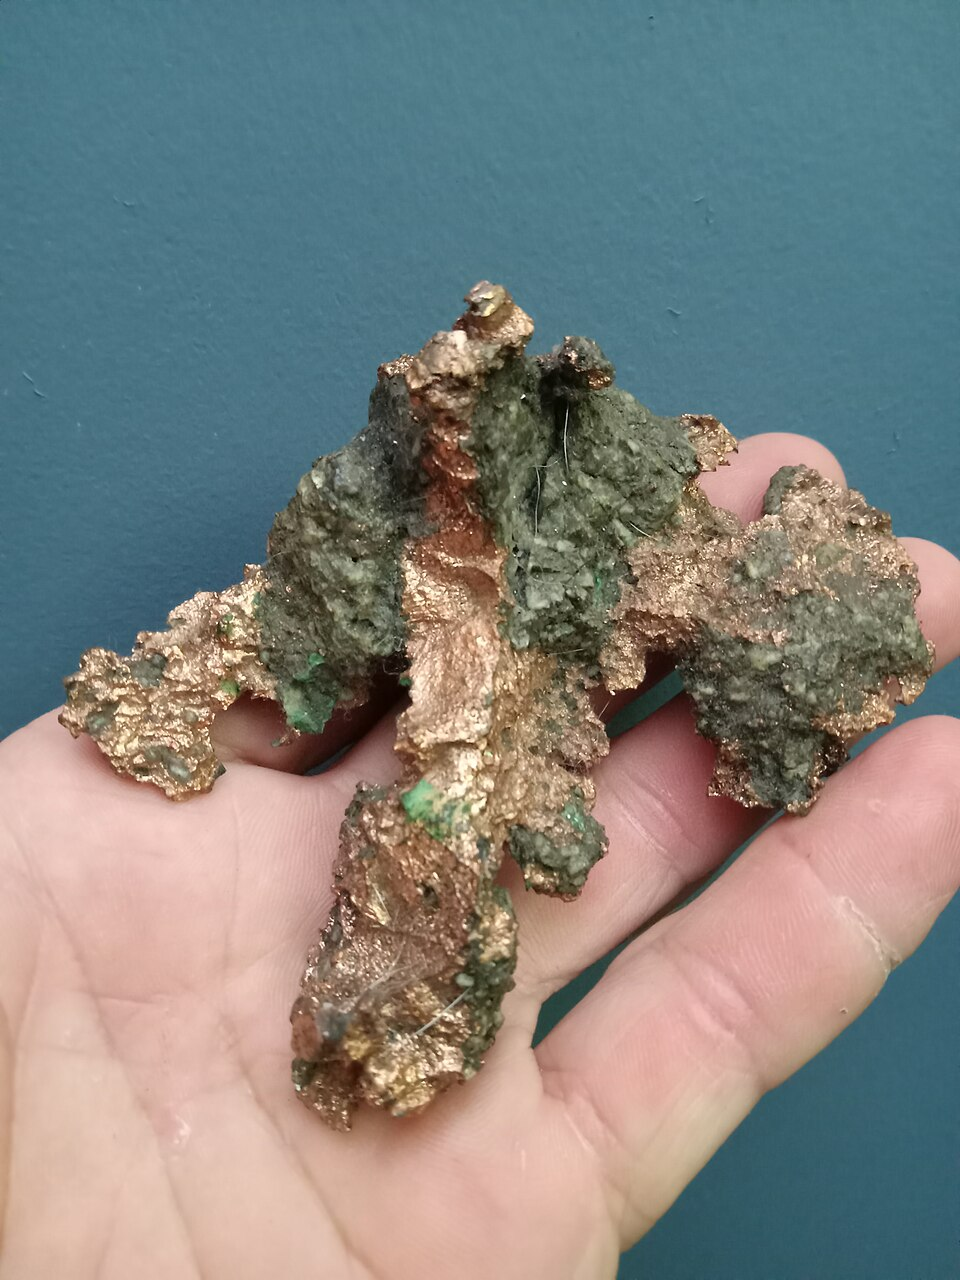
\includegraphics[width=0.36\linewidth]{images/book2/native-copper.jpg}

{\small 天然铜标本，其分枝状外形由\omterm{def:b1:crystals-metals:crystal}{晶体}生长形成；
内部金属是由\omterm{def:b1:crystals-metals:packings}{面心立方}晶粒组成的镶嵌结构。
图片：CC0（维基共享资源）。}
\end{omfigure}

\section{间隙位置}

\begin{definition}[间隙位置]\label{def:b1:crystals-metals:site}
\emph{间隙位置}\index{间隙位置}是\omterm{def:b1:crystals-metals:crystal}{晶体}中原子之间的空隙，
较小的原子可以占据其中。\emph{四面体间隙}\index{四面体间隙}位于
由四个原子组成的四面体中心，
\emph{八面体间隙}\index{八面体间隙}位于由六个原子组成的八面体中心。
间隙的\emph{可容纳性}\index{可容纳性}是指
能恰好放入该间隙中、且不会使周围原子相互推开的
最大球体的半径。
\end{definition}

\begin{proposition}[面心立方结构的间隙]\label{prop:b1:crystals-metals:sites}
\omterm{def:b1:crystals-metals:packings}{面心立方}\omterm{def:b1:crystals-metals:lattice}{晶胞}含 4 个\omterm{def:b1:crystals-metals:site}{八面体间隙}，位于立方体中心及
12 条棱的中点，另含 8 个\omterm{def:b1:crystals-metals:site}{四面体间隙}，位于
8 个边长为 $a/2$ 的小立方体中心。设原子半径为 $R$，且相邻原子相切，则
\omterm{def:b1:crystals-metals:site}{可容纳性}为
\[
  r_O = (\sqrt2 - 1)R \approx 0.414\,R, \qquad
  r_T = \left(\sqrt{\tfrac32} - 1\right)R \approx 0.225\,R .
\]
\end{proposition}

\begin{proof}
\omterm{def:b1:crystals-metals:site}{八面体间隙}数：$1 + 12 \times \frac14 = 4$，与原子数相等。
立方体中心到六个面心的距离为 $a/2$，故 $r_O + R = a/2$，
又 $a = 2\sqrt2 R$，因此 $r_O = (\sqrt2 - 1)R$。\omterm{def:b1:crystals-metals:site}{四面体间隙}：
边长为 $a/2$ 的小立方体中心位于其体对角线的一半处，
即 $\frac{a}{2}\cdot\frac{\sqrt3}{2} = \frac{a\sqrt3}{4}$，它到
相间顶点上四个原子的距离，故 $r_T + R = \frac{\sqrt3}{4}\,2\sqrt2\,R =
\sqrt{\tfrac32}\,R$.
\end{proof}

\begin{omfigure}
\tdplotsetmaincoords{60}{100}
\begin{tikzpicture}[tdplot_main_coords, font=\small]
  \pic {omcubeo={3}};
  \node[cellA=3.6mm] at (0,0,0) {};
  \node[cellsite=4mm, draw=omThm, fill=omThm!30] at (0,1.5,0) {};
  \node[cellA=3.6mm] at (0,3,0) {};
  \node[cellsite=4mm, draw=omThm, fill=omThm!30] at (0,0,1.5) {};
  \node[cellA=3.6mm] at (0,1.5,1.5) {};
  \node[cellsite=4mm, draw=omThm, fill=omThm!30] at (0,3,1.5) {};
  \node[cellsite=4mm, draw=omThm, fill=omThm!30] at (1.5,0,0) {};
  \node[cellA=3.6mm] at (0,0,3) {};
  \node[cellA=3.6mm] at (1.5,1.5,0) {};
  \node[cellsite=4mm, draw=omThm, fill=omThm!30] at (0,1.5,3) {};
  \node[cellsite=4mm, draw=omThm, fill=omThm!30] at (1.5,3,0) {};
  \node[cellA=3.6mm] at (0,3,3) {};
  \node[cellA=3.6mm] at (1.5,0,1.5) {};
  \node[cellsite=5mm, draw=omThm, fill=omThm!30] at (1.5,1.5,1.5) {};
  \node[cellA=3.6mm] at (1.5,3,1.5) {};
  \node[cellA=3.6mm] at (3,0,0) {};
  \node[cellsite=4mm, draw=omThm, fill=omThm!30] at (1.5,0,3) {};
  \node[cellsite=4mm, draw=omThm, fill=omThm!30] at (3,1.5,0) {};
  \node[cellA=3.6mm] at (1.5,1.5,3) {};
  \node[cellA=3.6mm] at (3,3,0) {};
  \node[cellsite=4mm, draw=omThm, fill=omThm!30] at (1.5,3,3) {};
  \node[cellsite=4mm, draw=omThm, fill=omThm!30] at (3,0,1.5) {};
  \node[cellA=3.6mm] at (3,1.5,1.5) {};
  \node[cellsite=4mm, draw=omThm, fill=omThm!30] at (3,3,1.5) {};
  \node[cellA=3.6mm] at (3,0,3) {};
  \node[cellsite=4mm, draw=omThm, fill=omThm!30] at (3,1.5,3) {};
  \node[cellA=3.6mm] at (3,3,3) {};
  \node[below] at (1.5,1.5,-1.5) {八面体间隙（红色）};
\end{tikzpicture}
\hspace{1.2cm}
\begin{tikzpicture}[tdplot_main_coords, font=\small]
  \pic {omcubeo={3}};
  \node[cellA=3.6mm] at (0,0,0) {};
  \node[cellA=3.6mm] at (0,3,0) {};
  \node[cellA=3.6mm] at (0,1.5,1.5) {};
  \node[cellsite=4mm, fill=omDef!30] at (0.75,0.75,0.75) {};
  \node[cellsite=4mm, fill=omDef!30] at (0.75,2.25,0.75) {};
  \node[cellA=3.6mm] at (0,0,3) {};
  \node[cellA=3.6mm] at (1.5,1.5,0) {};
  \node[cellsite=4mm, fill=omDef!30] at (0.75,0.75,2.25) {};
  \node[cellA=3.6mm] at (0,3,3) {};
  \node[cellA=3.6mm] at (1.5,0,1.5) {};
  \node[cellsite=4mm, fill=omDef!30] at (0.75,2.25,2.25) {};
  \node[cellsite=4mm, fill=omDef!30] at (2.25,0.75,0.75) {};
  \node[cellA=3.6mm] at (1.5,3,1.5) {};
  \node[cellA=3.6mm] at (3,0,0) {};
  \node[cellsite=4mm, fill=omDef!30] at (2.25,2.25,0.75) {};
  \node[cellA=3.6mm] at (1.5,1.5,3) {};
  \node[cellA=3.6mm] at (3,3,0) {};
  \node[cellsite=4mm, fill=omDef!30] at (2.25,0.75,2.25) {};
  \node[cellsite=4mm, fill=omDef!30] at (2.25,2.25,2.25) {};
  \node[cellA=3.6mm] at (3,1.5,1.5) {};
  \node[cellA=3.6mm] at (3,0,3) {};
  \node[cellA=3.6mm] at (3,3,3) {};
  \draw[omDef!70!black, thin] (0,0,0) -- (0.75,0.75,0.75) -- (1.5,1.5,0)
    (0.75,0.75,0.75) -- (1.5,0,1.5) (0.75,0.75,0.75) -- (0,1.5,1.5);
  \node[below] at (1.5,1.5,-1.5) {四面体间隙（蓝色）};
\end{tikzpicture}

{\small FCC \omterm{def:b1:crystals-metals:lattice}{晶胞}的\omterm{def:b1:crystals-metals:site}{间隙位置}。左：位于
中心的\omterm{def:b1:crystals-metals:site}{八面体间隙}，以及位于棱中点的\omterm{def:b1:crystals-metals:site}{八面体间隙}（每个由四个\omterm{def:b1:crystals-metals:lattice}{晶胞}共享）。右：
八个\omterm{def:b1:crystals-metals:site}{四面体间隙}位于八个小立方体的中心，
图中画出其中一个并与其四个原子相连。}
\end{omfigure}

\section{金属键与合金}

\begin{definition}[金属键]\label{def:b1:crystals-metals:metallic-bond}
在\emph{金属键}\index{金属键}中，每个金属原子
将其\omterm{def:b1:quantum-numbers:configuration}{价电子}交给整个\omterm{def:b1:crystals-metals:crystal}{晶体}：固体是由阳离子构成的\omterm{def:b1:crystals-metals:lattice}{晶格}，
这些阳离子浸没在电子之中，这些电子不专属于任何特定原子，
并可在\omterm{def:b1:crystals-metals:crystal}{晶体}中自由运动。该键即阳离子与
这片共享电子云之间的吸引作用，它没有方向性。
\end{definition}

\begin{proposition}[金属的性质]\label{prop:b1:crystals-metals:properties}
\omterm{def:b1:crystals-metals:metallic-bond}{金属键}可解释金属的性质：可移动的电子
导电、导热，并反射光（即金属光泽）；由于\omterm{def:b1:crystals-metals:metallic-bond}{金属键}
没有方向性，原子层可彼此滑过而
不破坏\omterm{def:b1:crystals-metals:crystal}{晶体}（延展性、展性），而\omterm{def:b1:crystals-metals:packings}{密堆积}，
它使近邻数最多，是最常见的结构。
\end{proposition}
\admitted

\begin{definition}[合金]\label{def:b1:crystals-metals:alloy}
合金是由几种元素组成的金属固体。在
\emph{置换型合金}\index{置换型合金}中，加入元素的原子
取代\omterm{def:b1:crystals-metals:lattice}{晶格}上基体的原子，这要求两者
半径相差在约 15\,\% 以内（如铜与镍、铜与
锌构成黄铜）。在\emph{间隙型合金}\index{间隙型合金}中，
小原子（\ce{H}、\ce{C}、\ce{N}、\ce{B}）占据基体的
\omterm{def:b1:crystals-metals:site}{间隙位置}（如钢中的碳）。
\end{definition}

\begin{definition}[同素异形体]\label{def:b1:crystals-metals:allotropy}
同一元素的不同\omterm{def:b1:crystals-metals:crystal}{晶体}结构称为其
\emph{同素异形体}\index{同素异形体}。铁在
室温下为\omterm{def:b1:crystals-metals:packings}{体心立方}（$\alpha$-铁）；实测其在 \qty{1189}{K} 至
\qty{1661}{K} 之间为\omterm{def:b1:crystals-metals:packings}{面心立方}（$\gamma$-铁），而在 \qty{1662}{K} 时又为\omterm{def:b1:crystals-metals:packings}{体心立方}（$\delta$-铁），
直到熔点。碳以金刚石与石墨两种形式存在
（见\cref{ch:b1:crystals-ionic-covalent}）。
% ledger: lat:Fe-alpha, lat:Fe-gamma-1189, lat:Fe-gamma-1661,
% lat:Fe-delta-1662
\end{definition}

\begin{example}[钢]\label{ex:b1:crystals-metals:steel}
碳的\omterm{def:b1:periodicity:radius}{共价半径}为 \qty{77}{pm}（即金刚石中 \ce{C-C}
键长的一半），若不发生畸变，它对铁的\omterm{def:b1:crystals-metals:site}{间隙位置}而言过大，但
在 $\gamma$-铁中则小得多，其\omterm{def:b1:crystals-metals:site}{八面体间隙}最大。钢
是通过在高温 $\gamma$-铁中溶解碳制得的；淬火时，碳
随铁转变回体心结构而被截留，此结构会使
\omterm{def:b1:crystals-metals:crystal}{晶体}发生畸变，畸变后的\omterm{def:b1:crystals-metals:crystal}{晶体}很硬。
% ledger: lat:C-diamond (r = a sqrt3 / 8 = 77.2 pm)
\end{example}

\begin{remark}[铁的相变]\label{rem:b1:crystals-metals:iron-T}
\cref{def:b1:crystals-metals:allotropy}中的温度，即纯铁在
大气压强下的温度；溶解的碳会降低 $\gamma$-铁形成的温度，
这使钢易于加工。
合金的相图在本科二年级分册中研究。
\end{remark}

\section{练习}

\begin{exercise}[$\star$]\label{exo:b1:crystals-metals:1}
数一数简单立方\omterm{def:b1:crystals-metals:lattice}{晶胞}（仅顶点处有原子）、
\omterm{def:b1:crystals-metals:packings}{体心立方}\omterm{def:b1:crystals-metals:lattice}{晶胞}和\omterm{def:b1:crystals-metals:packings}{面心立方}\omterm{def:b1:crystals-metals:lattice}{晶胞}中的原子数，并给出每种\omterm{def:b1:crystals-metals:lattice}{晶胞}的\omterm{def:b1:crystals-metals:coordination}{配位数}。
\end{exercise}

\begin{exercise}[$\star$]\label{exo:b1:crystals-metals:2}
证明简单立方结构（原子沿棱相切）的\omterm{def:b1:crystals-metals:compactness}{堆积率}为 $\pi/6$，
并与\omterm{def:b1:crystals-metals:packings}{面心立方}和\omterm{def:b1:crystals-metals:packings}{体心立方}比较。
\end{exercise}

\begin{exercise}[$\star$]\label{exo:b1:crystals-metals:3}
铝为\omterm{def:b1:crystals-metals:packings}{面心立方}结构，$a = \qty{405.0}{pm}$。计算其原子半径和
密度（$M = \qty{26.98}{g/mol}$）。
% ledger: lat:Al, aw:Al
\end{exercise}

\begin{exercise}[$\star$]\label{exo:b1:crystals-metals:4}
钠为\omterm{def:b1:crystals-metals:packings}{体心立方}结构，$a = \qty{429.1}{pm}$。计算其原子半径和
密度（$M = \qty{22.99}{g/mol}$），并与实测值
\qty{0.97}{g/cm^3} 比较。
% ledger: lat:Na, rho:Na, aw:Na
\end{exercise}

\begin{exercise}[$\star\star$]\label{exo:b1:crystals-metals:5}
银为\omterm{def:b1:crystals-metals:packings}{面心立方}结构，其密度为 \qty{10.50}{g/cm^3}
（$M = \qty{107.87}{g/mol}$）。计算\omterm{def:b1:crystals-metals:lattice}{晶胞参数}和原子
半径。
% ledger: rho:Ag, aw:Ag
\end{exercise}

\begin{exercise}[$\star\star$]\label{exo:b1:crystals-metals:6}
证明在相切球构成的\omterm{def:b1:crystals-metals:packings}{六方密堆积}结构中 $c/a = \sqrt{8/3}$。
镁的 $a = \qty{320.9}{pm}$，$c = \qty{521.0}{pm}$。计算 $c/a$
及镁的密度（$M = \qty{24.31}{g/mol}$）。
% ledger: lat:Mg.a, lat:Mg.c, aw:Mg
\end{exercise}

\begin{exercise}[$\star\star$]\label{exo:b1:crystals-metals:7}
在棱长为 $a$ 的\omterm{def:b1:crystals-metals:packings}{面心立方}\omterm{def:b1:crystals-metals:lattice}{晶胞}中，给出属于该\omterm{def:b1:crystals-metals:lattice}{晶胞}的
4 个原子、4 个\omterm{def:b1:crystals-metals:site}{八面体间隙}和 8 个\omterm{def:b1:crystals-metals:site}{四面体间隙}的坐标。
每个原子分别对应多少个这样的间隙？
\end{exercise}

\begin{exercise}[$\star\star$]\label{exo:b1:crystals-metals:8}
铜和镍均为\omterm{def:b1:crystals-metals:packings}{面心立方}结构，$a = \qty{361.5}{pm}$，
$a = \qty{352.4}{pm}$。计算它们的原子半径。二者
可以任意比例形成\omterm{def:b1:crystals-metals:alloy}{置换型合金}，试说明理由。
氢是很小的原子，它与金属能形成哪一类合金？
% ledger: lat:Cu, lat:Ni
\end{exercise}

\begin{exercise}[$\star\star$]\label{exo:b1:crystals-metals:9}
钨为\omterm{def:b1:crystals-metals:packings}{体心立方}结构，$a = \qty{316.5}{pm}$。计算其半径、
密度（$M = \qty{183.84}{g/mol}$）以及
\qty{1}{cm^3} 中的原子数。
% ledger: lat:W, aw:W
\end{exercise}

\begin{exercise}[$\star\star\star$]\label{exo:b1:crystals-metals:10}
在\omterm{def:b1:crystals-metals:packings}{体心立方}结构中，\omterm{def:b1:crystals-metals:site}{八面体间隙}位于每个面的中心
（以及每条棱的中点），\omterm{def:b1:crystals-metals:site}{四面体间隙}位于
每个面上的 $(\frac{a}{2}, \frac{a}{4}, 0)$ 处。证明它们的
\omterm{def:b1:crystals-metals:site}{可容纳性}分别为 $r_O = \frac{2 - \sqrt3}{4}\,a$ 和
$r_T = \frac{\sqrt5 - \sqrt3}{4}\,a$，并将其表示为
$R$ 的分数。哪一种间隙更大？
\end{exercise}

\begin{exercise}[$\star\star\star$]\label{exo:b1:crystals-metals:11}
某金属\omterm{def:b1:crystals-metals:crystal}{晶体}的每个立方\omterm{def:b1:crystals-metals:lattice}{晶胞}含 $Z$ 个原子，棱长为 $a$。证明
\omterm{def:b1:crystals-metals:compactness}{堆积率}可写为 $C = \frac{4\pi R^3 Z}{3a^3}$，再证明
$C = \frac{\pi\rho N_A}{6M}\,(2R)^3$。应用于铜（$R = \qty{127.8}{pm}$，
$\rho = \qty{8.93}{g/cm^3}$），验证其值为 $0.74$。
\end{exercise}

\begin{exercise}[$\star\star\star$]\label{exo:b1:crystals-metals:12}
金为\omterm{def:b1:crystals-metals:packings}{面心立方}结构，$a = \qty{407.8}{pm}$；银为\omterm{def:b1:crystals-metals:packings}{面心立方}结构，
$a = \qty{408.6}{pm}$。金与银可以任意比例混合。估算
两者各占 50\,\% 原子的合金的\omterm{def:b1:crystals-metals:lattice}{晶胞参数}
（取平均值），并计算其密度（$M(\ce{Au}) = \qty{196.97}{g/mol}$，
$M(\ce{Ag}) = \qty{107.87}{g/mol}$）。
% ledger: lat:Au, lat:Ag, aw:Au, aw:Ag
\end{exercise}

\section{问题：为什么钢能容纳碳}

\begin{problem}[{周末问题——相变温度（约 1190\,K）上下的铁，
其原子之间的间隙，
以及为碳留出的空间}]
\label{pb:b1:crystals-metals:1}
数据：$M(\ce{Fe}) = \qty{55.845}{g/mol}$，$M(\ce{C}) = \qty{12.011}{g/mol}$，
$N_A = \qty{6.022e23}{mol^{-1}}$。室温下，$\alpha$-铁为\omterm{def:b1:crystals-metals:packings}{体心立方}结构，
\omterm{def:b1:crystals-metals:lattice}{晶胞参数} $a = \qty{286.65}{pm}$。在 \qty{1189}{K}（刚高于相变温度）时，
低于相变温度时仍存在的 $\alpha$-铁测得
$a = \qty{289.8}{pm}$，而\omterm{def:b1:crystals-metals:packings}{面心立方}结构的 $\gamma$-铁 $a = \qty{363.9}{pm}$。
金刚石为立方结构，$a = \qty{356.68}{pm}$，每个碳原子与另外四个碳原子相接，
位于主对角线的四分之一处。
% ledger: lat:Fe-alpha, lat:Fe-alpha-1189, lat:Fe-gamma-1189,
% lat:C-diamond, aw:Fe, aw:C, const:NA

\medskip
\noindent\textbf{第一部分——室温下的 $\alpha$-铁。}
\begin{enumerate}
  \item 一个\omterm{def:b1:crystals-metals:packings}{体心立方}\omterm{def:b1:crystals-metals:lattice}{晶胞}含有多少个原子？其
        \omterm{def:b1:crystals-metals:coordination}{配位数}是多少？
  \item 原子沿哪条直线相切？计算一个铁原子的
        半径。
  \item 计算 $\alpha$-铁的密度。
  \item \qty{1}{cm^3} 的 $\alpha$-铁中有多少个铁原子？
  \item 计算\omterm{def:b1:crystals-metals:packings}{体心立方}结构的\omterm{def:b1:crystals-metals:compactness}{堆积率}。
  \item 与实测密度 \qty{7.87}{g/cm^3} 比较。
% ledger: rho:Fe
\end{enumerate}

\medskip
\noindent\textbf{第二部分——跨越相变。}
\begin{enumerate}[resume]
  \item 计算铁原子在 $\alpha$-铁和
        $\gamma$-铁中的半径，温度为 \qty{1189}{K}。
  \item 计算每个相中每个原子所占的体积。
  \item 哪一相的密度更大？分别计算两者的密度。
  \item 加热时，棒材从 $\alpha$ 相转变为
        $\gamma$ 相时，体积变化了百分之几？
  \item 该结果是否与两种结构的
        \omterm{def:b1:crystals-metals:compactness}{堆积率}相符？
\end{enumerate}

\medskip
\noindent\textbf{第三部分——$\alpha$-铁中的空穴。}
\begin{enumerate}[resume]
  \item 由金刚石结构，计算碳的\omterm{def:b1:periodicity:radius}{共价半径}。
  \item 在 \qty{1189}{K} 的\omterm{def:b1:crystals-metals:packings}{体心立方} $\alpha$-铁中，计算\omterm{def:b1:crystals-metals:site}{八面体间隙}
        的\omterm{def:b1:crystals-metals:site}{可容纳性}，$r_O = \frac{2 - \sqrt3}{4}\,a$。
  \item 计算\omterm{def:b1:crystals-metals:site}{四面体间隙}的\omterm{def:b1:crystals-metals:site}{可容纳性}，$r_T = \frac{\sqrt5 -
        \sqrt3}{4}\,a$。
  \item 与碳的半径比较，碳原子周围的
        \omterm{def:b1:crystals-metals:lattice}{晶格}必须发生怎样的变化？
  \item 解释碳为何只能微量地溶解于
        $\alpha$-铁中。
\end{enumerate}

\medskip
\noindent\textbf{第四部分——$\gamma$-铁中的空穴。}
\begin{enumerate}[resume]
  \item $\gamma$-铁的\omterm{def:b1:crystals-metals:packings}{面心立方}\omterm{def:b1:crystals-metals:lattice}{晶胞}中，按每个铁原子计
        含有多少个\omterm{def:b1:crystals-metals:site}{八面体间隙}？
  \item 计算 $\gamma$-铁\omterm{def:b1:crystals-metals:site}{四面体间隙}的\omterm{def:b1:crystals-metals:site}{可容纳性}。
  \item 若所有\omterm{def:b1:crystals-metals:site}{八面体间隙}都被碳填满，
        则该固体的化学式及碳的质量分数是多少？
  \item 若每十个\omterm{def:b1:crystals-metals:site}{八面体间隙}中有一个被碳填充，
        则碳的质量分数是多少？
  \item 解释为何钢是通过将碳溶解于热的铁中制得的。
  \item 计算能放入
        $\gamma$-铁\omterm{def:b1:crystals-metals:site}{八面体间隙}中的最大球的半径。
\end{enumerate}
\end{problem}
